\documentclass[a4paper,10pt]{article}
\usepackage[utf8]{inputenc}
\usepackage{geometry} 	%pour les marges
\usepackage{color} %pour la definition de nouvelles couleurs
\usepackage{graphicx} %pour ajouter des images 
\usepackage[final]{pdfpages} 
\usepackage[francais]{babel} % ``Franciser '' le document
\usepackage{lscape}
\usepackage	
  [colorlinks=false, urlcolor=red, breaklinks, pagebackref, citebordercolor={0 0 0}, 
  filebordercolor={0 0 0}, linkbordercolor={0 0 0}, pagebordercolor={0 0 0}, 
  runbordercolor={0 0 0}, urlbordercolor={0 0 0}, pdfborder={0 0 0}]
	{hyperref} % Ajouter le package des lien redirigeant sans les encadrer 
\usepackage{eurosym}
\usepackage{dirtree}
\usepackage{comment}

%couleurs pour les morceaux de code
\definecolor{codegreen}{rgb}{0,0.6,0}
\definecolor{codered}{rgb}{1,0.1,0.2}
\definecolor{codegray}{rgb}{0.5,0.5,0.5}
\definecolor{codepurple}{rgb}{0.58,0,0.82}
\definecolor{backcolour}{rgb}{0.95,0.95,0.92}
 

%modificaion des marges
\geometry{hmargin=2.5cm,vmargin=3cm}


%opening
\title{Architecture Logicielle : UML Reverse}

\title{\bfseries Document d’Architecture Logicielle \\Projet UML Reverse}
\geometry{hmargin=2.5cm,vmargin=3cm}
\begin{document}
\maketitle
\begin{center}
\begin{tabular}{ll}
  Version~: & 0.1\\[.5em]
  Date~: & \date{\today}\\[.5em]
  Rédigé par~:  & Yohann \textsc{Henry}\\
		& Nabil \textsc{Belkhous}\\
		& Stephen \textsc{Cauchois}\\
		& Anthony \textsc{Godin}\\
		& Florian \textsc{Inchingolo}\\
		& Saad \textsc{Mrabet}\\
		& Nicolas \textsc{Meniel}\\
\end{tabular}
\end{center}

\newpage
\begin{center}
    \section*{Mises à jour}
    \begin{tabular}{|l|l|p{8cm}|}
        \hline{\textbf{Version}} & {\textbf{Date}} & {\textbf{Modifications réalisées}}\\\hline
        {0.3} & {20/05/2016} & {}\\\hline
        {0.2} & {22/01/2016} & {Architecture refaite dans l'intégralité}\\\hline
        {0.1} & {14/01/2016} & {Première version}\\\hline
    \end{tabular}
\end{center}

%Table of contents
\newpage
\tableofcontents
\newpage


\section{Objectif}
Ce document représente la structure générale du logiciel et les modèles de conception mis en oeuvre pour le réaliser.
Il est destiné aux membres de l'équipe de développment, notamment aux concepteurs, ainsi qu'aux superviseurs du projet.

\section{Les technologies utilisées}
Nous allons utiliser différentes technologies pour la construction du projet.
\newline
Le projet est développé en Java 1.8.
Le projet utilise :
\begin{itemize}
 \item \emph{JUnit} : Framework pour valider chaque classe par le biais de tests unitaires.
 \item \emph{Maven} : Un outil pour la gestion des dépendances de l'application.
 \item \emph{Antlr} : Un parser dans lequel nous pourrons définir les grammaires pour l'extraction des données d'un fichier java ou plantUml.
 \item \emph{OpenJFX} : Une bibliothèque graphique libre parfaite pour ce projet. La bibliothèque permet d'associer à une entité du CSS, ce qui simplifie fortement notre travail.
 \item \emph{SceneBuilder} : Logiciel permettant de créer des vues de façon ergonomique en drag and drop. Les vues sont créées en FXML.  
\end{itemize}

\section{Organisation des paquetages}

  \dirtree{%
    .1 src.
    .2 model.
    .3 diagram\DTcomment{Modèle des diagrammes}.
    .4 clazz.
    .5 visitor\DTcomment{Permet le parcours du diagramme de classe}.
    .4 common.
    .4 usecase.
    .5 visitor\DTcomment{Permet le parcours du diagramme de cas}.
    .4 util.
    .4 visitor\DTcomment{Visiteurs globaux. Choisit d'appeler un visiteur en particulier selon le type de diagramme}.
    .3 io.parser\DTcomment{Parseur de plantUML et Java en diagramme}.
    .3 project\DTcomment{Modèle d'un projet qui contient des diagrammes}.
    .3 util.
    .2 ui.
    .3 component\DTcomment{Contient les composants utilisés dans la vue}.
    .4 clazz.
    .4 common.
    .4 usecase.
    .3 view\DTcomment{Contient les vues principales de l'application avec leurs contrôleurs}.
    .4 clazz.
    .4 common.
    .4 usecase.
    .4 util.
    .2 util.
    .2 MainApp.java.
  }

  \section{Paquetage model}
    Le modèle est représenté par une classe principale : \textbf{Project}. 
    Cette classe va servir à réunir tous les diagrammes et les éléments communs 
    aux différents diagrammes.
    La sauvegarde et le chargement sont effectués par le biais d'une sérialisation/désérialisation 
    de cette classe et de son contenu.
    La plupart des fonctionnalitées ajoutées s'effectuent par le biais de visiteur qui appelleront 
    à leur tour les visiteurs spécifiques à chaque diagramme.
    
    \subsection{Eléments liés}
    Le projet contient les éléments pouvant être liés entre différents diagrammes.
    Actuellement, cela représente les \textbf{IObjectEntity} et les \textbf{IRelation}.
    En les stockant dans \textbf{Project}, chaque diagramme peut facilement récupérer 
    les informations de ces éléments, voir les lier fortement pour synchroniser les contenus.
    C'est ainsi que fonctionne le diagramme de classe. Par contre, le diagramme de cas n'utilise 
    en aucune façon la liaison d'élément.
    
    \subsection{Diagramme de classe}
    Le diagramme de classe (\textbf{IClassDiagram}) est relativement simple. 
    Pour la majorité de son travail, il ne s'agit que d'une vue des \textbf{IObjectEntity} 
    et des \textbf{IRelation}.
    Ces vues sont des éléments se contentant d'associer une boite de style (\textbf{StyleBox}) 
    à chaque élément pour ajouter des fonctionnalités esthétiques.
    Le diagramme peut aussi contenir des notes.
    
   \newpage
  \section{Paquetage ui}
    L'application s'appuie sur la structure JavaFX avec la classe applicative UmlReverseApp qui est composée d'un stage qui en suivant
    la hiérarchie JavaFX nous ammène au BorderPane. Le BorderPane nous servira de base pour les différents éléments de notre application,
    tel qu'une TreeFileManagerView, une MenuBar, un IDiagramEditor et un IDiagramMenu.
    \begin{center}
	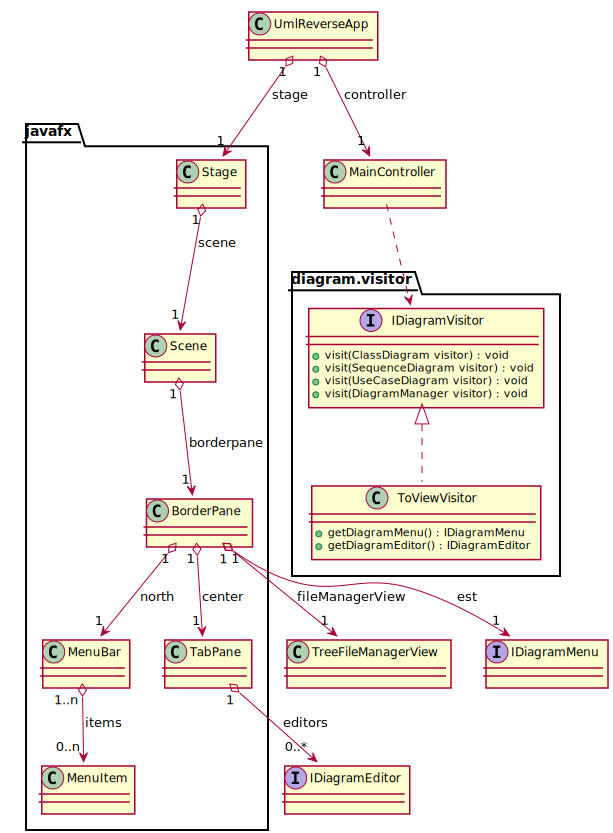
\includegraphics[width=10cm]{imgDAL/Vue.png}
    \end{center}
  
    Ce paquetage contient toutes les classes utilisées pour gérer la vue. Ces classes sont toujours associées à un contrôleur.
    Les vues sont codées en FXML grâce à un logiciel de construction de FXML (SceneBuilder). Chaque contrôleur aura le même nom
    que la vue associée avec le mot «~Controller~» ajouté à la fin.
    ui contient 2 paquetages :
    \begin{itemize}
    \item view : Contient les différentes vues intégrées dans l'application. Le paquetage contient également tous les contrôleurs associés à leur vue.
    \item component : Contient toutes les classes utilisées pour construire les vues. Ce sont leurs composants.
    \end{itemize}
    L'application graphique est l'association de plusieurs vues dans un BorderPane.
    
    \begin{center}
	\includegraphics[width=\textwidth]{imgDAL/maquette.png}
    \end{center}

  \subsection{La partie gauche}
    La partie gauche est séparée en deux verticalement. La partie supérieure présente le projet ouvert 
    et la liste des diagrammes qu’il contient, et permet de naviguer entre eux dans une vue hiérarchique 
    construite à partir du modèle. La partie inférieure affiche une liste des entités (classes, interfaces, 
    classes abstraites et énumérations) présentes dans le projet, et permet d'insérer dans le diagramme 
    courant toute entité qui n'y est pas déjà.
    
    \begin{center}
	\includegraphics[width=4cm]{imgDAL/partieGaucheVue.png}
    \end{center}
  \subsection{La partie centrale}
    La partie centrale sert à éditer graphiquement un diagramme. \\
    \textbf{\underline{Explication}}: Toutes les classes qui finissent par \textbf{Graphic} sont des 
    représentations graphiques des élements du modèle. Elles contiennent des écouteurs de souris sur 
    elles-mêmes pour pouvoir permettre aux utilisateurs de les modifier, ce qui modifiera le modèle directement.
    La modification du modèle modifie obligatoirement la vue du diagramme (les éléments graphiques donc) 
    grâce à des écouteurs sur le modèle.
    \newpage
    \subsubsection{Éditeur de diagramme}
	La partie MVC a été volontairement omise pour éviter de surcharger le diagramme de classe. 
	Elle sera en revanche implémentée dans les parties prévues.\\
	Dans les diagrammes ci-contre, les contrôleurs contrôleront les actions de \textbf{IDiagramEditor}. 
	Des pop-ups d'édition seront disponibles, elles seront placé dans les paquetages \textbf{dialog}.
	\subsubsection{Paquetages}
	
	  \begin{center}
	      \includegraphics[width=\textwidth]{imgDAL/DiagramEditor_EntityPackage3.png}
	  \end{center}
	  Voici toutes les entités présentes dans nos packages.
	  \newpage
	
	\subsubsection{Explications}
	  \begin{center}
	    \includegraphics[width=\textwidth]{imgDAL/demonstration.png}
	  \end{center}
      
          
\section{Paquetage main}
    Contient la classe qui lance l'application. C'est le point d'entrée. Il charge les différentes 
    vues du paquetage ui.view en les rassemblant toutes dans un BorderPane.
    
\section{Extensibilité}
  L'architecture a été pensée de façon à vérifier l'exigence \textbf{EXF\_70} (code modulaire, 
  ajout de nouvelles fonctionnalités possible dans le code).
  \paragraph{Modèle}
    Le modèle a été pensé de manière à facilement ajouter de nouveaux types de diagrammes. 
    Pour ce faire, le gestionnaire de diagramme ne se soucie pas du type de diagramme.
    La plupart des actions demandées sur un diagramme de manière extérieure au modèle se font par 
    le biais des visiteurs. Pour ajouter un nouveau type de diagramme, il suffit de créer une nouvelle 
    classe qui implémente \textbf{IDiagram} et de mettre à jour les visiteurs globaux.
  \paragraph{Partie gauche de l'application}
    Les différentes classes créées peuvent être héritées afin d'étendre leurs fonctionnalitées ainsi 
    que d'ajouter de nouveaux types de diagramme. 
    L'architecture des dossiers d'un projet a été pensée afin que l'ajout de nouveau type de fichier 
    pour la sauvegarde des diagrammes soit simple sans rendre les projets de cette version obsolètes.
  \paragraph{IDiagramEditor}
    Tout d'abord, l'ajout de nouveaux types de diagrammes a été pensé de façon à être possible et 
    facile à implémenter. 
    Pour ce faire, il suffit d'ajouter une nouvelle classe \textbf{XXXDiagramEditor}. 
    Cette nouvelle classe peut hériter \textbf{ADiagramEditor} si le nouveau type de diagramme peut posséder des notes.
    L'implémentation de celle-ci sera déjà faite. Les classes présentes dans le paquetage view.component.common 
    sont des classes qui peuvent être utilisées dans n'importe quel type de diagramme. Ce
    sont généralement des classes abstraites qui effectuent une partie du travail, ce qui évite de tout refaire à chaque fois.


\begin{comment}
  \subsection{model}
  Ce package contient l'intégralité du modèle. Il contient tous les packages et classes pour le travail métier.
  \subsubsection{util}
  Le code commun à tous les diagrammes
  \begin{center}
      \includegraphics[width=\textwidth]{imgDAL/util2.png}
  \end{center}
  \begin{landscape}
      \includegraphics[height=12cm]{imgDAL/utilDiagramme.png}
  \end{landscape}
  Ce package contient l'intégralité du code commun à chaque diagramme. 
  C'est aussi ici qu'on trouve la définition des boîtes de style.
  \subsubsection{visitor}
  Les visiteurs permettent l'ajout d'opérations homogènes à des entités d'un modèle sans couplage.
  \begin{center}
      \includegraphics[width=\textwidth]{imgDAL/visitor.png}
  \end{center}
  Ce package contient les visiteurs des diagrammes.
  \subsubsection{classDiagram}
  \begin{center}
      \includegraphics[width=\textwidth]{imgDAL/classDiagramUp.png}
  \end{center}
  \begin{center}
      \includegraphics[width=12cm]{imgDAL/classDiagramBottom.png}
  \end{center}
  Ce package contient le code pour stocker un diagramme de classe extrait à partir d'un fichier java. 
  A fortiori, il gère tout diagramme de classe en plantUml représentant un diagramme de classe valide en UML2.
  \subsubsection{sequenceDiagram}
  \begin{center}
      \includegraphics[width=\textwidth]{imgDAL/SequenceDiag.png}
  \end{center}
  \begin{center}
      \includegraphics[width=\textwidth]{imgDAL/SeqBlocksDiag.png}
  \end{center}
  Ce package contient le code pour stocker un diagramme de séquence. 
  Il gère tout diagramme de séquence en plantUml représentant un diagramme de séquence valide en UML2.
  \subsubsection{useCaseDiagram}
  \begin{center}
      \includegraphics[width=\textwidth]{imgDAL/UseCaseDiag.png}
  \end{center}
  Ce package contient le code pour stocker un diagramme de cas d'utilisation. 
  Il gère tout diagramme de cas d'utilisation en plantUml représentant un diagramme de séquence valide en UML2.
  \subsubsection{parser}
   Les imports
  \begin{center}
      \includegraphics[width=\textwidth]{imgDAL/parser.png}
  \end{center}
  Ce package contient les différents parsers qui seront utilisées pour extraire le style, le plantUml et le java.

  \subsection{ui}
  Ce package contient l'intégralité de la vue et des contrôleurs.
  \subsubsection{view}
  C'est dans ce package que se situe les différentes vues utilisées par l'application.
  \subsubsection{controllers}
  Ce package contient toutes les classes permettant la communication entre la vue et le modèle.
  \subsubsection{components}
  Les différents composants de l'ihm
  \begin{center}
      \includegraphics[width=\textwidth]{imgDAL/Component.png}
  \end{center}
  Ce package contient les composants qui seront utilisées par la vue.
  
\section{}
\end{comment}

\end{document}
